%%% Preamble starts here.
\documentclass{amsart}
%for the heading
\usepackage{fancyhdr, enumerate,multirow}
%for the picture. 
\usepackage{float}
\usepackage{tikz, calc}
%adjust the page width
\usepackage[margin=1in]{geometry}
\usepackage{xcolor}

\usepackage{array}   % for \newcolumntype macro
\newcolumntype{L}{>{$}l<{$}} % math-mode version of "l" column type


%% The next line says how the "vertex" style of nodes should look: drawn as small circles.
\tikzstyle{vertex}=[circle, draw, inner sep=0pt, minimum size=6pt,fill=white]
%%
%% Next, we make a \vertex command as a shorthand in place of \node[vertex} to get that style.
\newcommand{\vertex}{\node[vertex]}

\linespread{1.1}


%special commands for number sets
\def\RR{{\mathbb R}}
\def\NN{{\mathbb N}}
\def\ZZ{{\mathbb Z}}
\def\QQ{{\mathbb Q}}
\def\CC{{\mathbb C}}
\usepackage{soul}
\usepackage{color}
% header
\lhead{\sc  Senior Seminar: Homework 9}
\chead{\sc Stefano Fochesatto } 
\rhead{due: Friday 04/03/2020}
\cfoot{}
\pagestyle{fancy}

%%%% Main document starts here.

\begin{document}
\thispagestyle{fancy}
 
\begin{enumerate}
\item (Problem A:) Apply the Augmenting Path Algorithm to the graph, with matching, below until a maximum matching is found. Explicitly state M, U, S, T and the output of the Algorithm at each iteration. \\

\begin{center}
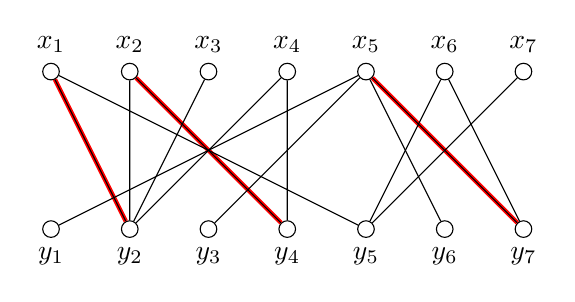
\begin{tikzpicture}
\foreach \i in {1,2,3,4,5,6,7}{
	\vertex (x\i) at (\i,2)[label=above:{$x_{\i}$}]{};
	\vertex (y\i) at (\i,0)[label=below:{$y_{\i}$}]{};
	}
\draw[red, ultra thick] (x1) -- (y2) (x2) -- (y4) (x5) --(y7);
\draw (x1) -- (y5) (x2)--(y2)(x3)--(y2) (x4)--(y2) (x4)--(y4) (x6)--(y5) (x5)--(y7) (x1)--(y2);
\draw (x5) -- (y3) (x5) -- (y1) (x5) -- (y6)  (x6)--(y7) (x2) -- (y4);
\draw (x7)--(y5);
\end{tikzpicture}
\end{center}

\textbf{Answer:} Note that if an edge is made green it is added to $M$. If an edge is made blue it is removed from $M$.\\
\begin{center}
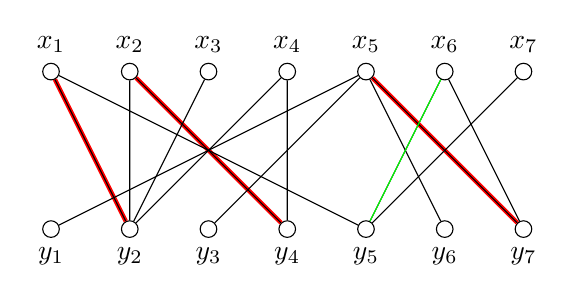
\begin{tikzpicture}
\foreach \i in {1,2,3,4,5,6,7}{
	\vertex (x\i) at (\i,
	2)[label=above:{$x_{\i}$}]{};
	\vertex (y\i) at (\i,0)[label=below:{$y_{\i}$}]{};
	}
\draw[red, ultra thick] (x1) -- (y2) (x2) -- (y4) (x5) --(y7);
\draw (x1) -- (y5) (x2)--(y2)(x3)--(y2) (x4)--(y2) (x4)--(y4) (x6)--(y5) (x5)--(y7) (x1)--(y2);
\draw (x5) -- (y3) (x5) -- (y1) (x5) -- (y6)  (x6)--(y7) (x2) -- (y4);
\draw (x7)--(y5);
\draw[green] (y5)--(x6);
\end{tikzpicture}
\end{center}
\noindent Iteration 1:\\
$M=\{x_1y_2, x_2y_4,x_5y_7\}$\\
$U=\{x_3,x_4,x_6,x_7\}$\\
$S=\{x_3,x_4,x_6,x_7,x_1(via-y_2), x_2(via-y_4) $\\
$T=\{y_2, y_4,y_5(unsaturated) $\\
Vertices Explored: $x_3, x_4,x_6$ \\
Output: M is not a maximum, and the algorithm would return the edge $y_5 x_6$.
\\\\

\begin{center}
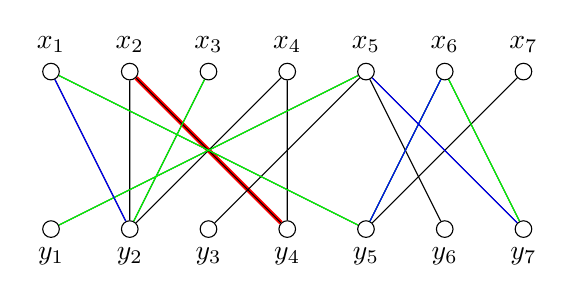
\begin{tikzpicture}
\foreach \i in {1,2,3,4,5,6,7}{
	\vertex (x\i) at (\i,2)[label=above:{$x_{\i}$}]{};
	\vertex (y\i) at (\i,0)[label=below:{$y_{\i}$}]{};
	}
\draw[red, ultra thick] (x2) -- (y4);
\draw (x1) -- (y5) (x2)--(y2)(x3)--(y2) (x4)--(y2) (x4)--(y4) (x6)--(y5) (x5)--(y7) (x1)--(y2);
\draw (x5) -- (y3) (x5) -- (y1) (x5) -- (y6)  (x6)--(y7) (x2) -- (y4);
\draw (x7)--(y5);
\draw[green] (y1) -- (x5)  (y7) -- (x6) -- (y5) -- (x1)  (y2) -- (x3);
\draw[blue] (x5) -- (y7)  (x6) -- (y5)  (x1) -- (y2);
\end{tikzpicture}
\end{center}
Iteration 2:\\
$M=\{x_1y_2, x_2y_4,x_5y_7, y_5,x_6 \}$\\
$U=\{x_3,x_4,x_7\}$\\
$S=\{x_3,x_4,x_7, x_1(via-y_2), x_2(via-y_4), x_6(via-y_5), x_5(via-y_7)$\\
$T=\{y_2, y_4, y_5, y_7, y_1(unsaturated)  $\\
Vertices Explored: $x_3, x_4, x_7, x_1, x_2, x_6, x_5$ \\
Output: M is not a maximum, and the algorithm would return the $M$-augmenting path $(y_1, x_5, y_7, x_6, y_5, x_1, y_2, x_3)$.
\\\\


\begin{center}
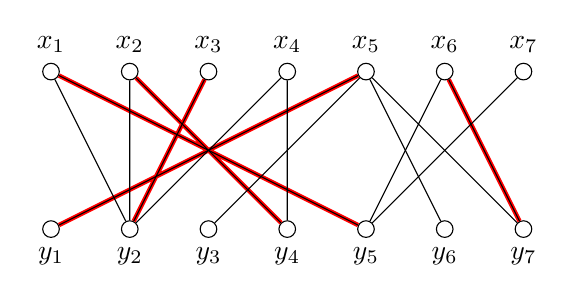
\begin{tikzpicture}
\foreach \i in {1,2,3,4,5,6,7}{
	\vertex (x\i) at (\i,2)[label=above:{$x_{\i}$}]{};
	\vertex (y\i) at (\i,0)[label=below:{$y_{\i}$}]{};
	}
\draw[red, ultra thick] (x2) -- (y4) (y1)--(x5) (y7) -- (x6) (y5) -- (x1) (y2) -- (x3);
\draw (x1) -- (y5) (x2)--(y2)(x3)--(y2) (x4)--(y2) (x4)--(y4) (x6)--(y5) (x5)--(y7) (x1)--(y2);
\draw (x5) -- (y3) (x5) -- (y1) (x5) -- (y6)  (x6)--(y7) (x2) -- (y4);
\draw (x7)--(y5);
\end{tikzpicture}
\end{center}
Iteration 3:\\
$M=\{(x_2,y_4 y_1,x_5 y_7,x_6 y_5,x_1 y_2,x_3 \}$\\
$U=\{x_4, x_7\}$\\
$S=\{x_4, x_7, x_3(via-y_2), x_2(via-y_4), x_1(via-y_5)  $\\
$T=\{y_2, y_4, y_5 $\\
Vertices explored: $x_4, x_7, x_3, x_2, x_1$ \\
Output: Since the algorithm fails to produce an augmenting path by Theorem 3.2.2 we can conclude that $M$ is a maximum matching and $R$ is a vertex cover size $|M|$ such that, $R = T \cup (X-S)$.

\vspace{1.5in}

\item (Problem B) Prove that if $M$ is a matching and $Q$ is a vertex cover, then $|M| \leq |Q|.$ Given an example of a graph in which $M$ is a maximum matching, $Q$ is a minimum vertex cover and $|M| < |Q|.$\\

\textbf{Proof:} (Direct) If we can prove that the largest size matching is still smaller than the smallest size vertex cover i.e. $\beta \geq \alpha'$ then $|M| \leq |Q|$ is immediate. Note that since no edge can cover two vertices of an independent set we know that $\beta' \geq \alpha$. By Lemma 3.1.21 we know that $\alpha = n - \beta$. By Theorem 3.1.22 we know that $\beta' = n - \alpha'$. Through substitution,
\begin{align*}
\beta' &\geq \alpha,\\
 n - \alpha' &\geq n - \beta,\\
  n +  \beta &\geq n + \alpha',\\
  \beta &\geq \alpha'.
\end{align*}
For an example consider a $K_3$ which has a maximum matching $|M| = 1$ and a minimum vertex cover $|Q| = 2$.

\vspace{1.5in}

\item (Problem 3.2.3) (Direct) Give an example of the stable matching problem with two job openings and two applicants in which there is more than one stable matching.
 
\textbf{Answer}: Consider the following preference table,
\begin{center}
\begin{tabular}{LLLLLLLLLLLLL LLLLLLLLLLLL }
\multicolumn{4}{c}{\text{Companies} \{u,v\}}&& \multicolumn{4}{c}{\text{Applicants} \{a,b\}}\\
u:&a&>&b& \quad \quad \quad &a:&v&>&u&\\
v:&b&>&a& \quad \quad \quad  &b:&u&>&v&\\
\end{tabular}
\end{center}
Since the table is so small, in one iteration of the Gale-Shapley Proposal Algorithm, with the companies proposing we get the matching: $(u,a)(v,b)$. However, running the same algorithm again with the applicants proposing returns the matching: $(a,v)(b,u)$. Note that these two matching are stable since there are no two elements $(x,y)$ such that $x \in Companies$ and $y \in Applicants$ where $both$, $x$ and $y$ would rather be matched with each other than their respective partners. 
\vspace{.5in}

\vspace{1.5in}

\item (Problem 3.2.4) Determine the stable matchings resulting from the Proposal Algorithm run with men proposing and with women proposing given the preference lists below.

\begin{center}
\begin{tabular}{LLLLLLLLLLLLL LLLLLLLLLLLL }
&\multicolumn{10}{c}{\text{Men  } \{u,v,w,x,y,z\}}&&& \multicolumn{10}{c}{\text{Women  } \{a,b,c,d,e,f\}}\\
u:&a&>&b&>&d&>&c&>&f&>&e& \quad \quad &a:&z&>&x&>&y&>&u&>&v&>&w\\
v:&a&>&b&>&c&>&f&>&e&>&d& \quad \quad &b:&y&>&z&>&w&>&x&>&v&>&u\\
w:&c&>&b&>&d&>&a&>&f&>&e& \quad \quad &c:&v&>&x&>&w&>&y&>&u&>&z\\
x:&c&>&a&>&d&>&b&>&e&>&f& \quad \quad &d:&w&>&y&>&u&>&x&>&z&>&v\\
y:&c&>&d&>&a&>&b&>&f&>&e& \quad \quad &e:&u&>&v&>&x&>&w&>&y&>&z\\
z:&d&>&e&>&f&>&c&>&b&>&a& \quad \quad &f:&u&>&w&>&x&>&v&>&z&>&y\\
\end{tabular}
\end{center}
\vspace{.5in}
\textbf{Answer:}\\
Iteration 0: Every male proposes to their first preference. If a woman receives only one proposal they must accept, and If they have more than one proposal, they accept the male that is highest in their preference list. Proposals that are accepted are marked in green, otherwise the proposal is rejected and is marked in red. 

\begin{center}
\begin{tabular}{LLLLLLLLLLLLL LLLLLLLLLLLL }
u:&\textcolor{green}{a}&>&b&>&d&>&c&>&f&>&e& \quad \quad &a:&z&>&x&>&y&>&\textcolor{green}{u}&>&\textcolor{red}{v}&>&w\\
v:&\textcolor{red}{a}&>&b&>&c&>&f&>&e&>&d& \quad \quad &b:&y&>&z&>&w&>&x&>&v&>&u\\
w:&\textcolor{red}{c}&>&b&>&d&>&a&>&f&>&e& \quad \quad &c:&v&>&\textcolor{green}{x}&>&\textcolor{red}{w}&>&\textcolor{red}{y}&>&u&>&z\\
x:&\textcolor{green}{c}&>&a&>&d&>&b&>&e&>&f& \quad \quad &d:&w&>&y&>&u&>&x&>&\textcolor{green}{z}&>&v\\
y:&\textcolor{red}{c}&>&d&>&a&>&b&>&f&>&e& \quad \quad &e:&u&>&v&>&x&>&w&>&y&>&z\\
z:&\textcolor{green}{d}&>&e&>&f&>&c&>&b&>&a& \quad \quad &f:&u&>&w&>&x&>&v&>&z&>&y\\
\end{tabular}
\end{center}
\vspace{.25in}

Iteration 1+: Every unpaired man proposes to the woman that is highest in his preference list. 
\begin{center}
\begin{tabular}{LLLLLLLLLLLLL LLLLLLLLLLLL }
u:&\textcolor{green}{a}&>&b&>&d&>&c&>&f&>&e& \quad \quad &a:&z&>&x&>&y&>&\textcolor{green}{u}&>&\textcolor{red}{v}&>&w\\
v:&\textcolor{red}{a}&>&\textcolor{red}{b}&>&c&>&f&>&e&>&d& \quad \quad &b:&y&>&z&>&\textcolor{green}{w}&>&x&>&\textcolor{red}{v}&>&u\\
w:&\textcolor{red}{c}&>&\textcolor{green}{b}&>&d&>&a&>&f&>&e& \quad \quad &c:&v&>&\textcolor{green}{x}&>&\textcolor{red}{w}&>&\textcolor{red}{y}&>&u&>&z\\
x:&\textcolor{green}{c}&>&a&>&d&>&b&>&e&>&f& \quad \quad &d:&w&>&\textcolor{green}{y}&>&u&>&x&>&\textcolor{red}{z}&>&v\\
y:&\textcolor{red}{c}&>&\textcolor{green}{d}&>&a&>&b&>&f&>&e& \quad \quad &e:&u&>&v&>&x&>&w&>&y&>&z\\
z:&\textcolor{red}{d}&>&e&>&f&>&c&>&b&>&a& \quad \quad &f:&u&>&w&>&x&>&v&>&z&>&y\\
\end{tabular}
\end{center}
\vspace{.25in}

Iteration 2: Proposal $(x,c)$ is rejected in favor of $(v,c)$. Proposal $(z,e)$ is accepted.
\begin{center}
\begin{tabular}{LLLLLLLLLLLLL LLLLLLLLLLLL }
u:&\textcolor{green}{a}&>&b&>&d&>&c&>&f&>&e& \quad \quad &a:&z&>&x&>&y&>&\textcolor{green}{u}&>&\textcolor{red}{v}&>&w\\
v:&\textcolor{red}{a}&>&\textcolor{red}{b}&>&\textcolor{green}{c}&>&f&>&e&>&d& \quad \quad &b:&y&>&z&>&\textcolor{green}{w}&>&x&>&\textcolor{red}{v}&>&u\\
w:&\textcolor{red}{c}&>&\textcolor{green}{b}&>&d&>&a&>&f&>&e& \quad \quad &c:&\textcolor{green}{v}&>&\textcolor{red}{x}&>&\textcolor{red}{w}&>&\textcolor{red}{y}&>&u&>&z\\
x:&\textcolor{red}{c}&>&a&>&d&>&b&>&e&>&f& \quad \quad &d:&w&>&\textcolor{green}{y}&>&u&>&x&>&\textcolor{red}{z}&>&v\\
y:&\textcolor{red}{c}&>&\textcolor{green}{d}&>&a&>&b&>&f&>&e& \quad \quad &e:&u&>&v&>&x&>&w&>&y&>&\textcolor{green}{z}\\
z:&\textcolor{red}{d}&>&\textcolor{green}{e}&>&f&>&c&>&b&>&a& \quad \quad &f:&u&>&w&>&x&>&v&>&z&>&y\\
\end{tabular}
\end{center}
\vspace{.25in}


Iteration 3: Proposal $(u,a)$ is rejected in favor of $(x,a)$.
\begin{center}
\begin{tabular}{LLLLLLLLLLLLL LLLLLLLLLLLL }
u:&\textcolor{red}{a}&>&b&>&d&>&c&>&f&>&e& \quad \quad &a:&z&>&\textcolor{green}{x}&>&y&>&\textcolor{red}{u}&>&\textcolor{red}{v}&>&w\\
v:&\textcolor{red}{a}&>&\textcolor{red}{b}&>&\textcolor{green}{c}&>&f&>&e&>&d& \quad \quad &b:&y&>&z&>&\textcolor{green}{w}&>&x&>&\textcolor{red}{v}&>&u\\
w:&\textcolor{red}{c}&>&\textcolor{green}{b}&>&d&>&a&>&f&>&e& \quad \quad &c:&\textcolor{green}{v}&>&\textcolor{red}{x}&>&\textcolor{red}{w}&>&\textcolor{red}{y}&>&u&>&z\\
x:&\textcolor{red}{c}&>&\textcolor{green}{a}&>&d&>&b&>&e&>&f& \quad \quad &d:&w&>&\textcolor{green}{y}&>&u&>&x&>&\textcolor{red}{z}&>&v\\
y:&\textcolor{red}{c}&>&\textcolor{green}{d}&>&a&>&b&>&f&>&e& \quad \quad &e:&u&>&v&>&x&>&w&>&y&>&\textcolor{green}{z}\\
z:&\textcolor{red}{d}&>&\textcolor{green}{e}&>&f&>&c&>&b&>&a& \quad \quad &f:&u&>&w&>&x&>&v&>&z&>&y\\
\end{tabular}
\end{center}
\vspace{.25in}

Iteration 4: Proposal $(u,b)$ is rejected.
\begin{center}
\begin{tabular}{LLLLLLLLLLLLL LLLLLLLLLLLL }
u:&\textcolor{red}{a}&>&\textcolor{red}{b}&>&d&>&c&>&f&>&e& \quad \quad &a:&z&>&\textcolor{green}{x}&>&y&>&\textcolor{red}{u}&>&\textcolor{red}{v}&>&w\\
v:&\textcolor{red}{a}&>&\textcolor{red}{b}&>&\textcolor{green}{c}&>&f&>&e&>&d& \quad \quad &b:&y&>&z&>&\textcolor{green}{w}&>&x&>&\textcolor{red}{v}&>&\textcolor{red}{u}\\
w:&\textcolor{red}{c}&>&\textcolor{green}{b}&>&d&>&a&>&f&>&e& \quad \quad &c:&\textcolor{green}{v}&>&\textcolor{red}{x}&>&\textcolor{red}{w}&>&\textcolor{red}{y}&>&u&>&z\\
x:&\textcolor{red}{c}&>&\textcolor{green}{a}&>&d&>&b&>&e&>&f& \quad \quad &d:&w&>&\textcolor{green}{y}&>&u&>&x&>&\textcolor{red}{z}&>&v\\
y:&\textcolor{red}{c}&>&\textcolor{green}{d}&>&a&>&b&>&f&>&e& \quad \quad &e:&u&>&v&>&x&>&w&>&y&>&\textcolor{green}{z}\\
z:&\textcolor{red}{d}&>&\textcolor{green}{e}&>&f&>&c&>&b&>&a& \quad \quad &f:&u&>&w&>&x&>&v&>&z&>&y\\
\end{tabular}
\end{center}
\vspace{.25in}

Iteration 5: Proposal $(u,d)$ is rejected.
\begin{center}
\begin{tabular}{LLLLLLLLLLLLL LLLLLLLLLLLL }
u:&\textcolor{red}{a}&>&\textcolor{red}{b}&>&\textcolor{red}{d}&>&c&>&f&>&e& \quad \quad &a:&z&>&\textcolor{green}{x}&>&y&>&\textcolor{red}{u}&>&\textcolor{red}{v}&>&w\\
v:&\textcolor{red}{a}&>&\textcolor{red}{b}&>&\textcolor{green}{c}&>&f&>&e&>&d& \quad \quad &b:&y&>&z&>&\textcolor{green}{w}&>&x&>&\textcolor{red}{v}&>&\textcolor{red}{u}\\
w:&\textcolor{red}{c}&>&\textcolor{green}{b}&>&d&>&a&>&f&>&e& \quad \quad &c:&\textcolor{green}{v}&>&\textcolor{red}{x}&>&\textcolor{red}{w}&>&\textcolor{red}{y}&>&u&>&z\\
x:&\textcolor{red}{c}&>&\textcolor{green}{a}&>&d&>&b&>&e&>&f& \quad \quad &d:&w&>&\textcolor{green}{y}&>&\textcolor{red}{u}&>&x&>&\textcolor{red}{z}&>&v\\
y:&\textcolor{red}{c}&>&\textcolor{green}{d}&>&a&>&b&>&f&>&e& \quad \quad &e:&u&>&v&>&x&>&w&>&y&>&\textcolor{green}{z}\\
z:&\textcolor{red}{d}&>&\textcolor{green}{e}&>&f&>&c&>&b&>&a& \quad \quad &f:&u&>&w&>&x&>&v&>&z&>&y\\
\end{tabular}
\end{center}
\vspace{.25in}

Iteration 6: Proposal $(u,c)$ is rejected.
\begin{center}
\begin{tabular}{LLLLLLLLLLLLL LLLLLLLLLLLL }
u:&\textcolor{red}{a}&>&\textcolor{red}{b}&>&\textcolor{red}{d}&>&\textcolor{red}{c}&>&f&>&e& \quad \quad &a:&z&>&\textcolor{green}{x}&>&y&>&\textcolor{red}{u}&>&\textcolor{red}{v}&>&w\\
v:&\textcolor{red}{a}&>&\textcolor{red}{b}&>&\textcolor{green}{c}&>&f&>&e&>&d& \quad \quad &b:&y&>&z&>&\textcolor{green}{w}&>&x&>&\textcolor{red}{v}&>&\textcolor{red}{u}\\
w:&\textcolor{red}{c}&>&\textcolor{green}{b}&>&d&>&a&>&f&>&e& \quad \quad &c:&\textcolor{green}{v}&>&\textcolor{red}{x}&>&\textcolor{red}{w}&>&\textcolor{red}{y}&>&\textcolor{red}{u}&>&z\\
x:&\textcolor{red}{c}&>&\textcolor{green}{a}&>&d&>&b&>&e&>&f& \quad \quad &d:&w&>&\textcolor{green}{y}&>&\textcolor{red}{u}&>&x&>&\textcolor{red}{z}&>&v\\
y:&\textcolor{red}{c}&>&\textcolor{green}{d}&>&a&>&b&>&f&>&e& \quad \quad &e:&u&>&v&>&x&>&w&>&y&>&\textcolor{green}{z}\\
z:&\textcolor{red}{d}&>&\textcolor{green}{e}&>&f&>&c&>&b&>&a& \quad \quad &f:&u&>&w&>&x&>&v&>&z&>&y\\
\end{tabular}
\end{center}
\vspace{.25in}


Iteration 7: Proposal $(u,f)$ is accepted. All males are in a stable pair and the algorithm terminates.
\begin{center}
\begin{tabular}{LLLLLLLLLLLLL LLLLLLLLLLLL }
u:&\textcolor{red}{a}&>&\textcolor{red}{b}&>&\textcolor{red}{d}&>&\textcolor{red}{c}&>&\textcolor{green}{f}&>&e& \quad \quad &a:&z&>&\textcolor{green}{x}&>&y&>&\textcolor{red}{u}&>&\textcolor{red}{v}&>&w\\
v:&\textcolor{red}{a}&>&\textcolor{red}{b}&>&\textcolor{green}{c}&>&f&>&e&>&d& \quad \quad &b:&y&>&z&>&\textcolor{green}{w}&>&x&>&\textcolor{red}{v}&>&\textcolor{red}{u}\\
w:&\textcolor{red}{c}&>&\textcolor{green}{b}&>&d&>&a&>&f&>&e& \quad \quad &c:&\textcolor{green}{v}&>&\textcolor{red}{x}&>&\textcolor{red}{w}&>&\textcolor{red}{y}&>&\textcolor{red}{u}&>&z\\
x:&\textcolor{red}{c}&>&\textcolor{green}{a}&>&d&>&b&>&e&>&f& \quad \quad &d:&w&>&\textcolor{green}{y}&>&\textcolor{red}{u}&>&x&>&\textcolor{red}{z}&>&v\\
y:&\textcolor{red}{c}&>&\textcolor{green}{d}&>&a&>&b&>&f&>&e& \quad \quad &e:&u&>&v&>&x&>&w&>&y&>&\textcolor{green}{z}\\
z:&\textcolor{red}{d}&>&\textcolor{green}{e}&>&f&>&c&>&b&>&a& \quad \quad &f:&\textcolor{green}{u}&>&w&>&x&>&v&>&z&>&y\\
\end{tabular}
\end{center}
\vspace{.25in}
The Proposal Algorithm when the men are proposing returns the following matching: 
\begin{equation*}
(u,f) (v,c) (w, b) (x,a) (y,d) (z,e)
\end{equation*}





\item (Problem 3.2.11) Prove that if man $x$ is paired with woman $a$ is some stable matching, then $a$ does not reject $x$ in the Gale-Shipley Proposal Algorithm with men proposing. Conclude that among all stable matchings, \emph{every} man is happiest in the matching produced by this algorithm. The definition of "happiest" is to be paired with the woman of highest rank for which a stable matching is possible. (Hint: Consider the first occurrence of such a rejection.) \\


\textbf{Answer} (Contradiction:) Suppose that man $x$ is paired with a woman $a$ in some stable matching, and $a$ does reject $x$ in favor of $x'$ in the Gale-Shipley (GS) Proposal Algorithm with men proposing. 
Note that in our algorithm woman $a$ would only reject man $x$ in favor of $x'$ if $x'$ is higher in the $a$-preference list. Also note that in our algorithm, man $x'$ will only propose to $a$ if all other women above $a$ in the $x'$-preference list have rejected $x'$. Thus it must follow that $a$ has $x'$ higher in the preference list than $x$ and that $x'$ can only be paired with $a$ and women lower than $a$ in the $x'$-preference list. Thus any matching with $x,a$ wouldn't be stable because it would contain an unstable pair $(x',a)$\\
Suppose that the GS returns a stable matching with $(x,a)$. We know that $a$ is the women highest in the $x$-preference list where a stable match is possible, since every women higher than $a$ in the preference list would have had to reject $x$ in favor of a more suitable matching. (If we were to match $x$ with anyone higher than $a$ on the preference list it would result in an unstable matching.)



\end{enumerate}

\end{document}
